\section{Evaluation}

\subsection{ml-curves}
Show convergence of different data sets
\begin{figure}[t] % [htb]
  \centering
  \epsfig{file=plots/ppx-amazon.eps, width=\columnwidth}
  %\caption{}
  \label{fig-ppx-cpu}
\end{figure}

\begin{figure}[t] % [htb]
  \centering
  \epsfig{file=plots/ppx-dblp.eps, width=\columnwidth}
  %\caption{}
  \label{fig-ppx-cpu}
\end{figure}

  \begin{figure}[t] % [htb]
  \centering
  \epsfig{file=plots/ppx-friendster.eps, width=\columnwidth}
  %\caption{}
  \label{fig-ppx-cpu}
\end{figure}

\begin{figure}[t] % [htb]
  \centering
  \epsfig{file=plots/ppx-lj.eps, width=\columnwidth}
  %\caption{}
  \label{fig-ppx-cpu}
\end{figure}

\begin{figure}[t] % [htb]
  \centering
  \epsfig{file=plots/ppx-youtube.eps, width=\columnwidth}
  %\caption{}
  \label{fig-ppx-cpu}
\end{figure}

\subsection{sweep-over-K-fixed-np}
\begin{figure}[t] % [htb]
  \centering
  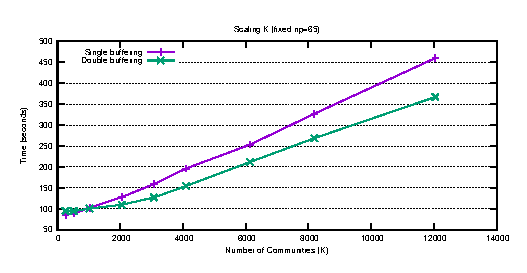
\epsfig{file=plots/sweep-over-K-fixed-np.eps, width=\columnwidth}
  %\caption{}
  \label{fig-ppx-cpu}
\end{figure}



\subsection{sweep-over-K-proportional-np}
Weak scaling

\begin{figure}[t] % [htb]
  \centering
  
\epsfig{file=plots/sweep-over-K-proportional-np.eps, width=\columnwidth}
  %\caption{}
  \label{fig-ppx-cpu}
\end{figure}

\subsection{sweep-over-np-fixed-K}
Strong scaling

\begin{figure}[t] % [htb]
  \centering
  \epsfig{file=plots/sweep-over-np-fixed-K.eps, width=\columnwidth}
  %\caption{}
  \label{fig-ppx-cpu}
\end{figure}

\subsection{hpc-cloud}
Scale up vs scale out
\begin{figure}[t] % [htb]
  \centering
  
\epsfig{file=plots/hpc-cloud.eps, width=\columnwidth}
  %\caption{}
  \label{fig-ppx-cpu}
\end{figure}

